\chapter{Proposed Methodology}

%\section{Modules}

%The system is divided into three modules :\\
%(1) Registration\\
%(2) Request Procedure\\
%(3) Administration

\section{Overview of the Proposed System}

The project involves the development of a user-friendly software tool that utilizes Optical Character Recognition (OCR) technology to convert scanned images of answer papers into Excel sheets. The software tool operates by capturing a picture of the front page of the answer sheet using a camera as input. It is then passed through a program to extract the table and its cells from the input image. These cells are passed to an OCR model made using the TensorFlow library to accurately convert the handwritten marks to digital text.

\begin{figure}[htbp]
  \centering
  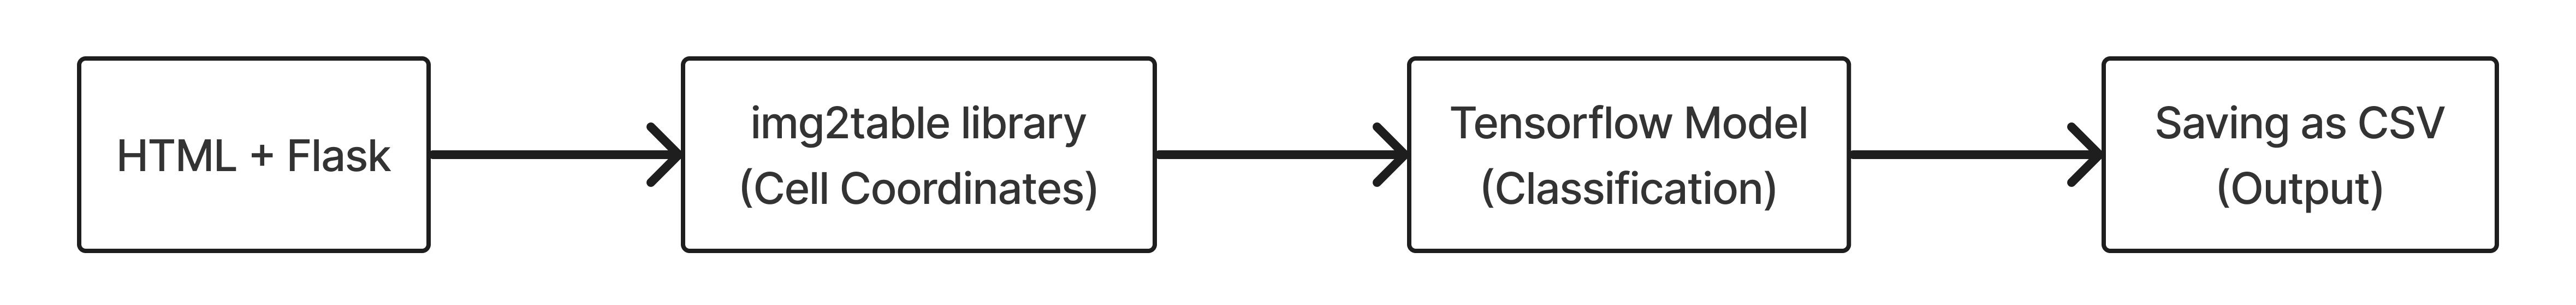
\includegraphics[width=\textwidth]{Images/System_in_four_steps.png}
  \caption{Our system in four steps}
\end{figure}

\noindent The extracted marks are then processed (removing unwanted columns and adding additional columns) to make it in an appropriate format and the end result is a comprehensive Excel sheet that faithfully represents the original content of the answer papers.

\clearpage

\subsection{Working of the system}

Our application features a professional and efficient user interface, developed using HTML and Flask. Designed to enhance interactivity and performance, this interface serves as the entry point for teachers to interact seamlessly. The central camera icon enables users to quickly open the camera and capture images of answer sheets, streamlining the process. This intuitive design fosters a professional environment, empowering teachers with a streamlined approach to their tasks. Figure 3.2 is the image of our interface.

\begin{figure}[h!]
    \centering
    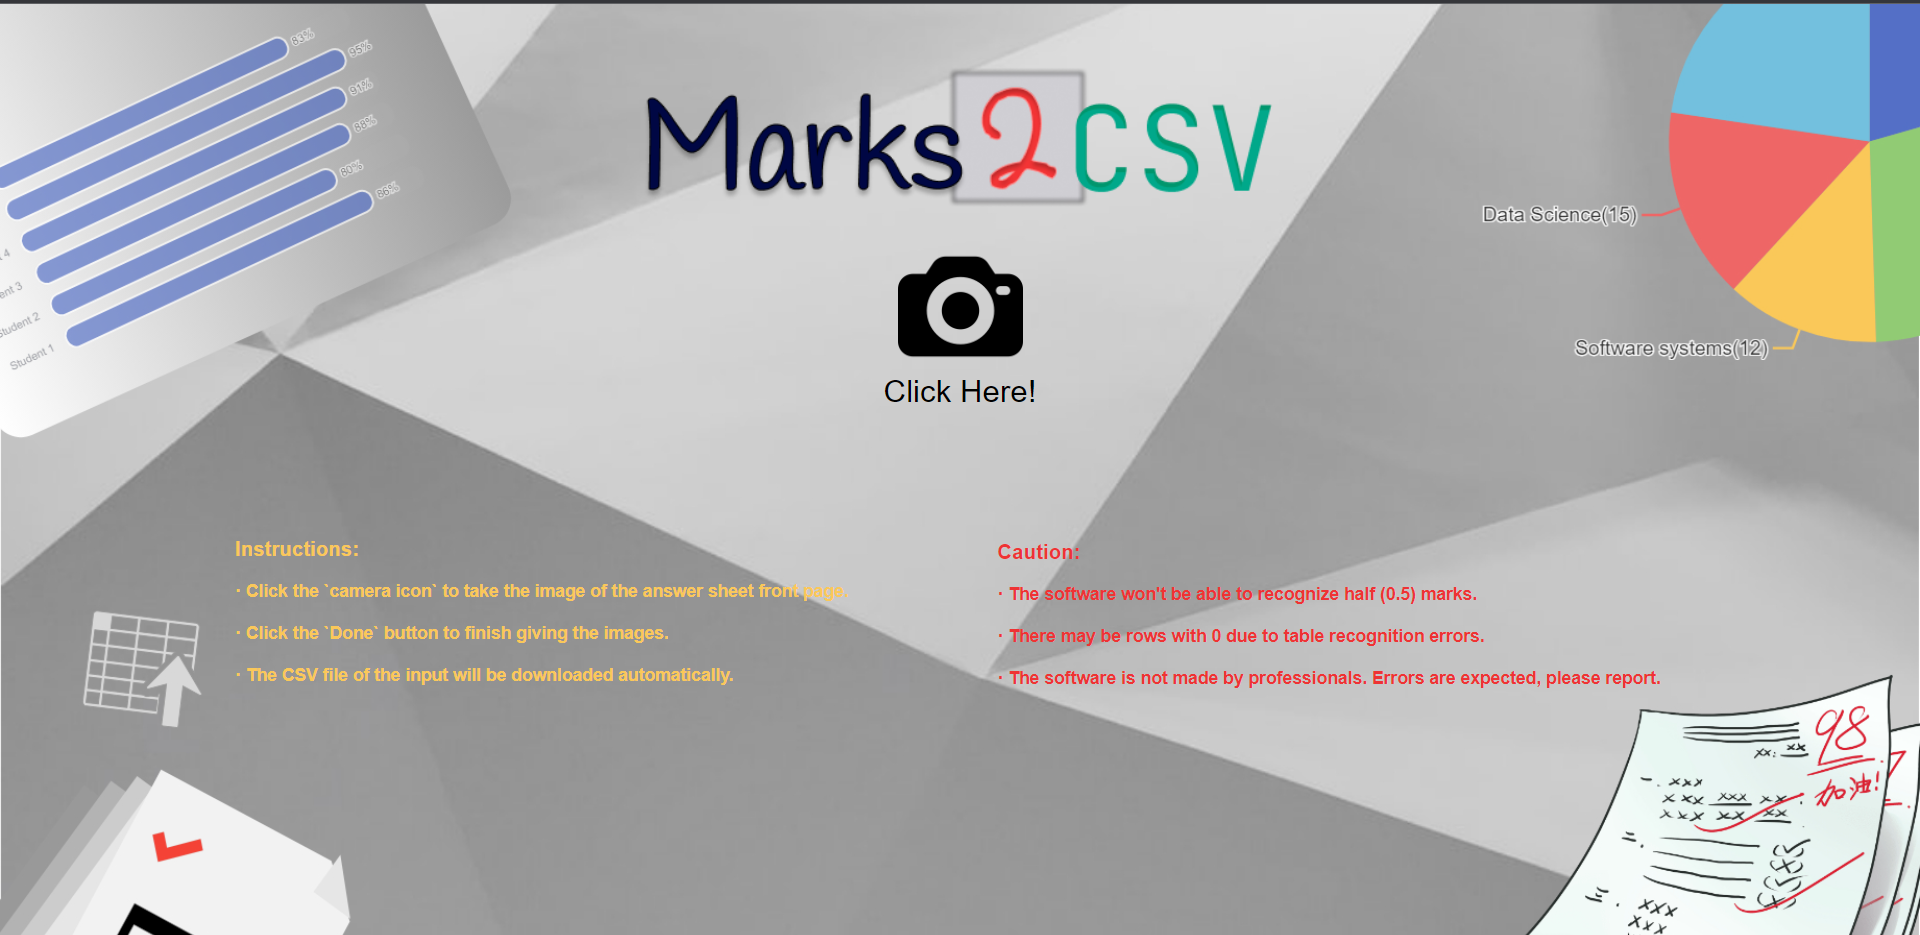
\includegraphics[width=0.8\textwidth]{Images/results/interface.png}
    \caption{Marks2CSV Interface}
\end{figure}

\noindent The input images are processed by the img2table library to extract the cell coordinates. Figure 3.3 shows the recognized table structure.

\begin{figure}[h!]
    \centering
    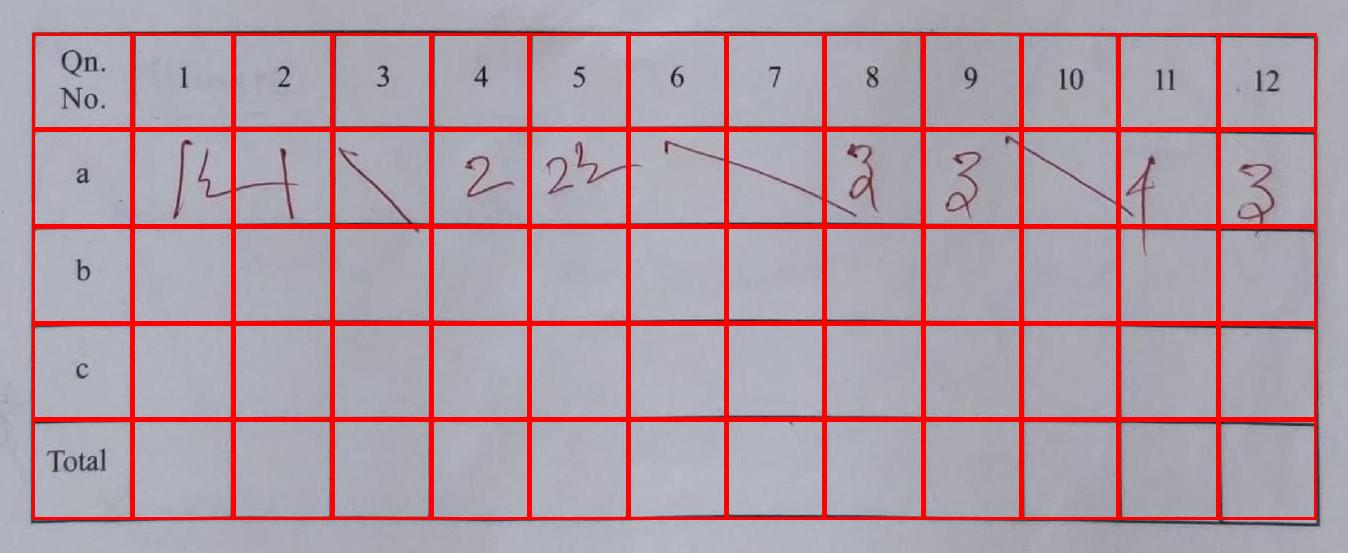
\includegraphics[width=0.8\textwidth]{Images/results/Img_with_redlines.jpg}
    \caption{Table Detection Output}
\end{figure}

\clearpage

\noindent Once the image is processed by the img2table library, the table cells are cropped based on these coordinates and forwarded to our image classification model. Figure 3.4 depicts the classification time taken by our model for each individual image, showcasing our model's exceptional speed and efficiency. Our model is specifically designed to prioritize speed without compromising accuracy. It boasts an impressive capability to process five images in a mere 18 seconds, showcasing its remarkable performance.

\begin{figure}[htbp]
    \centering
{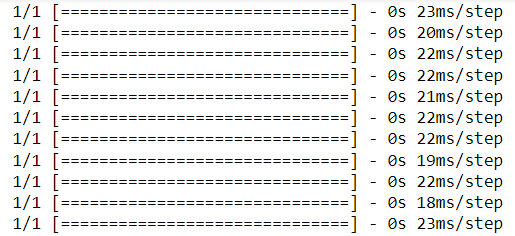
\includegraphics[scale=0.5, width=0.7\textwidth]{Images/results/TF_model_Running.png}}
  \caption{TensorFlow OCR model classifying images (Average time: 21ms)}
\end{figure}

\noindent After the classification process, the model's output is incorporated into a dictionary to store the marks of individual students. Following this, additional coding is applied for post-processing, which includes the removal of columns with identical entries. The resulting refined output is then provided in the form of a CSV file (refer to Figure 3.5). Notably, this CSV file is automatically downloaded through the application's interface, enabling seamless access to the finalized output on your local system.

\begin{figure}[htbp]
    \centering
{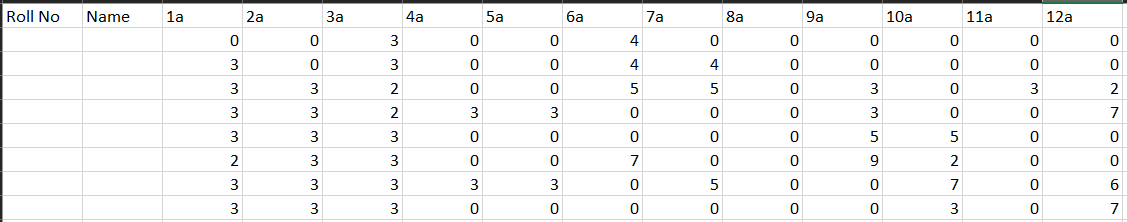
\includegraphics[width=1\textwidth]{Images/results/csv_output.png}}
  \caption{Output CSV File}
\end{figure}

\clearpage

\section{Block Diagram}

\subsection{Overall working of the system}

\noindent
The camera acquires a list of images that we require. From these images, we attempt to detect the table structure of the mark dataframe. This is done by a table detection algorithm, where the table is divided into cells and each cell's coordinates are stored in an ordered dictionary. From this ordered dictionary, we remove the first and last rows and sent the modified data to the TensorFlow OCR model for classification. The classification results are in the form of a dataframe, from which we remove the first column. Thus we flatten the dataframe properly and add the values to the marks dictionary. These values in the dictionary are transformed into a CSV file to obtain our final output.

\vspace{2 cm}

\begin{figure}[htbp]
  \centering
  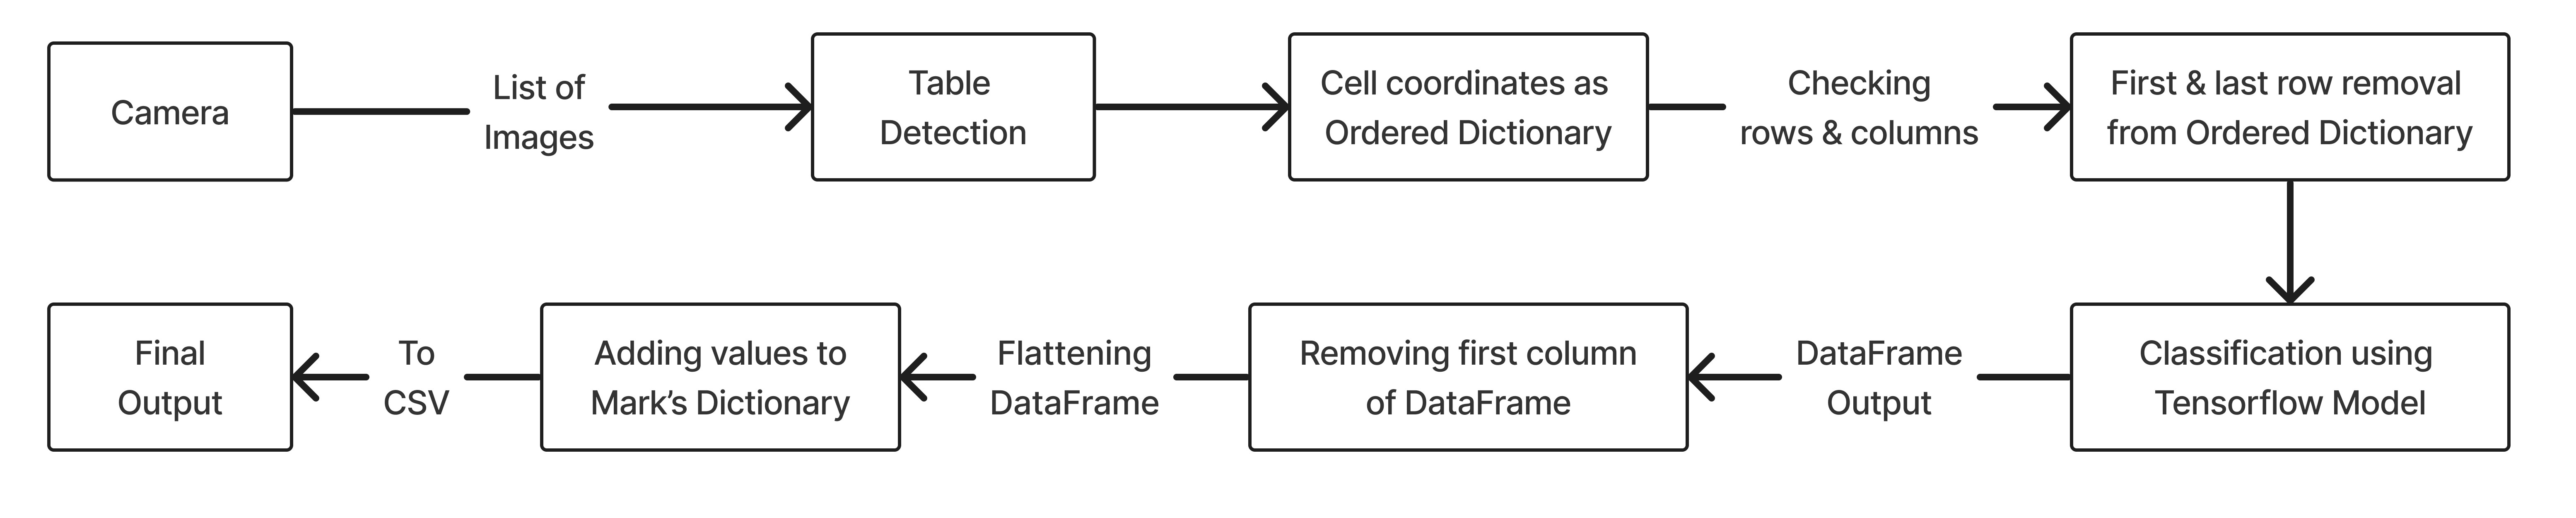
\includegraphics[width=1\textwidth]{Images/Dataset/Overall_Working_Of_System.jpg}
  \caption{Overall working of our system}
\end{figure}

\clearpage

\subsection{Data Collection}

\noindent Initially, we collected 614 images from college answer sheets. We were able to draw out the fact that this data was insufficient to train our model properly. So we acquired 21,600 images from a public Kaggle dataset. As per our project requirements, we removed image classes of numbers 8 and 9 from this dataset to get 17,454 images. Thus we finally achieved a collection of 18,068 as our new dataset.

\begin{figure}[h!]
    \centering
    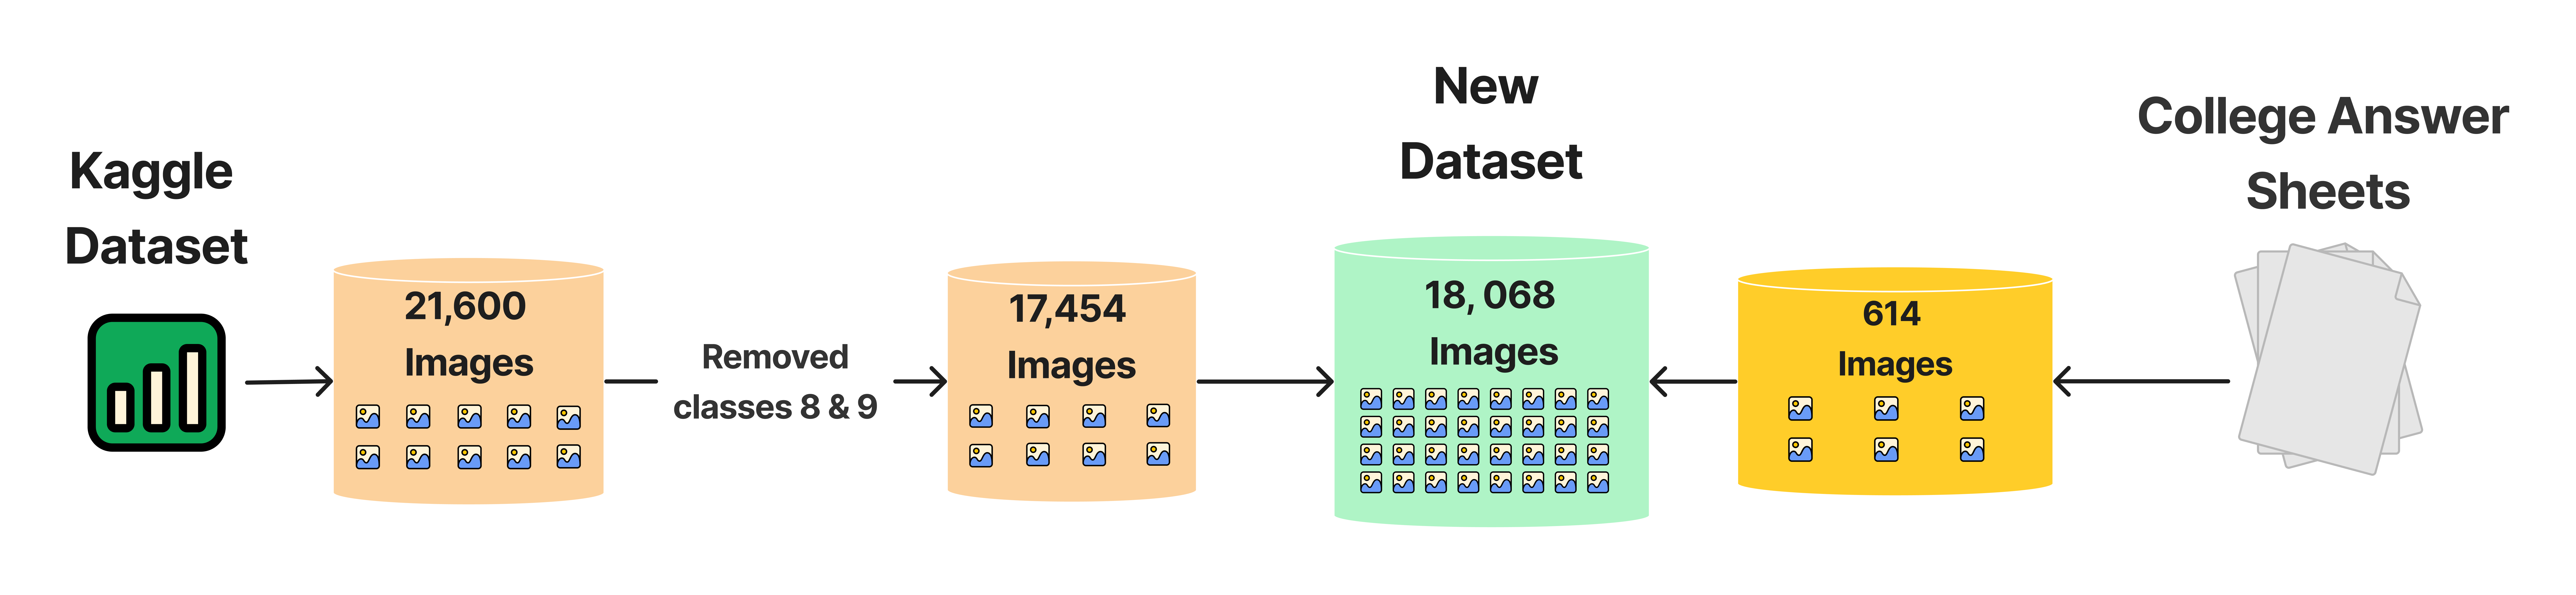
\includegraphics[width=\textwidth]
    {Images/Dataset/Dataset_Counts.png}
    \caption{Dataset Collection}
\end{figure}

\begin{figure}[h!]
    \centering
{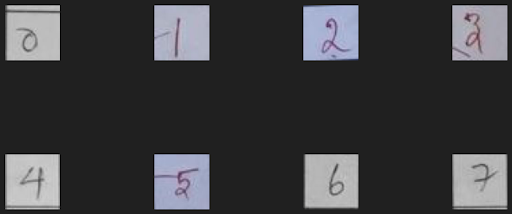
\includegraphics[width=0.6\textwidth]{Images/Dataset/Clg_ans_sheet.png}}
  \caption{Mark cells of college answer sheets}
\end{figure} 

\begin{figure}[h!]
  \centering
  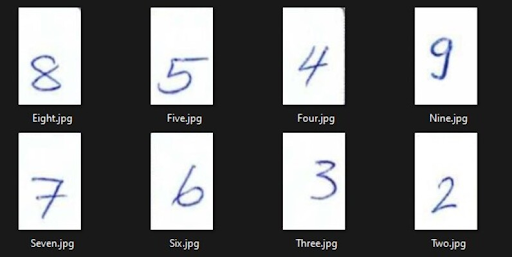
\includegraphics[width=0.6\textwidth]{Images/Dataset/Kaggle_Dataset_Header.png}
  \caption{Kaggle Dataset}
\end{figure} 

\clearpage

\subsection{Feature Extraction}

In the process of automated marks extraction, a crucial feature to be extracted is the mark associated with each cell of the table. A table extraction algorithm is employed to achieve this, which facilitates the extraction of marks from each cell when the entire table is detected. The algorithm operates by identifying the boundaries of the table and dividing it into square dimensions, representing individual cells.

\noindent Once the table is successfully detected and divided into cells, the marks extraction process begins. Each cell is isolated, and the algorithm focuses on extracting the mark contained within it. This is where the Convolutional Neural Network (CNN) model comes into play. The extracted cell is passed through the CNN model, which has been trained to classify and interpret the marks present within the cells accurately.  

\noindent In conclusion, the process of marks extraction from table cells involves the utilization of a table extraction algorithm and a CNN model. The algorithm enables the identification and isolation of individual cells within the table, allowing for the extraction of marks from each cell. The CNN model plays a vital role in accurately classifying and interpreting the marks within the cells. The inclusion of exception checking within the algorithm ensures e\noindent rror handling and robustness in cases where the expected number of cells is not detected. By incorporating these components and mechanisms, the automated marks extraction system achieves reliable and accurate results, facilitating streamlined data processing and analysis in educational assessment processes.

 \subsection{Classification/Prediction}

 In the marks extraction process, the classification and prediction of marks are performed by employing a Convolutional Neural Network (CNN). The CNN model is trained to categorize input images into nine distinct classes, ranging from 0 to 7, along with an additional class representing a null cell (empty cell). The objective of the CNN model is to predict the numerical equivalent of the image cell or identify it as null if it is empty.

\begin{figure}[htbp]
    \centering
    \subfigure[]{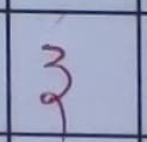
\includegraphics[width=0.25\textwidth,height=0.25\textwidth]{Images/mark_cells/good_mark_cell_1.png}}
    \hfill
    \subfigure[]{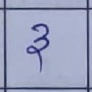
\includegraphics[width=0.25\textwidth,height=0.25\textwidth]{Images/mark_cells/good_mark_cell_2.png}}
    \caption{Cells with mark written correctly}
    
    \vspace{\floatsep}
    
    \subfigure[]{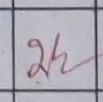
\includegraphics[width=0.25\textwidth,height=0.25\textwidth]{Images/mark_cells/half_mark_cell_1.png}}
    \hfill
    \subfigure[]{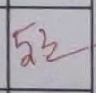
\includegraphics[width=0.25\textwidth,height=0.25\textwidth]{Images/mark_cells/half_mark_cell_2.png}}
    \caption{Cells with half marks (unable to detect)}
    
    \vspace{\floatsep}
    
    \subfigure[]{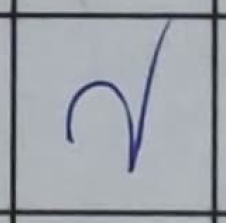
\includegraphics[width=0.25\textwidth,height=0.25\textwidth]{Images/mark_cells/unrecog_mark_cell_1.png}}
    \hfill
    \subfigure[]{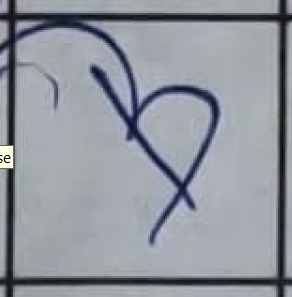
\includegraphics[width=0.25\textwidth,height=0.25\textwidth]{Images/mark_cells/unrecog_mark_cell_2.png}}
    \caption{Cells with hard-to-recognize marks (may give false result)}

    \vspace{\floatsep}

    \subfigure[]{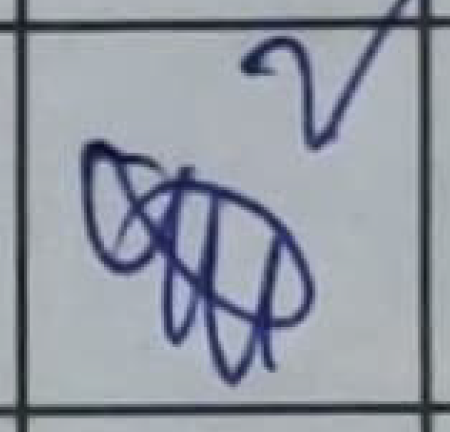
\includegraphics[width=0.25\textwidth,height=0.25\textwidth]{Images/mark_cells/cut_and_correction_mark_cell_1.png}}
    \hfill
    \subfigure[]{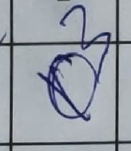
\includegraphics[width=0.25\textwidth,height=0.25\textwidth]{Images/mark_cells/cut_and_correction_mark_cell_2.png}}
    \caption{Cells with cuts \& corrections (unable to detect)}

\end{figure}

\noindent During the prediction phase, the CNN model takes an input image, typically representing a cell from a table, and processes it through its layers. Through the intricate architecture and learned weights, CNN analyzes the image's features and extracts meaningful representations. These representations are then utilized for classification and prediction purposes.

\noindent The CNN model has been trained on a comprehensive dataset, encompassing various examples of marked cells and null cells. By learning from this diverse set of inputs, the model gains the ability to accurately classify and predict the numerical values of marked cells or identify them as null if they are empty.

\noindent To ensure the correct sequence of marks, the extracted predictions are stored in a dictionary structure. The dictionary keys correspond to the table-detected cells, enabling the marks to be associated with their respective positions within the table. This ensures that the predicted cell values are stored in the correct sequence, maintaining the integrity and accuracy of the marks extraction process.

\noindent By predicting all the cell values before receiving the next input, the CNN model ensures efficient and consistent processing. This approach enables the system to swiftly extract and store the predicted marks in their corresponding positions, facilitating streamlined data management and subsequent analysis.

\noindent In summary, the classification and prediction in the marks extraction process are accomplished through the use of a CNN model. The CNN categorizes image cells into nine classes, representing numerical values from 0 to 7, and a null class for empty cells. The model leverages its learned representations to accurately predict the values of marked cells or identify them as null. The extracted predictions are stored in a dictionary, associating the predicted marks with their respective table positions. This methodology allows for efficient and accurate extraction of marks.
 

\section{Summary}

We use a simple interface built with HTML and Flask that supports the working of a camera device to capture the images that we require. The captured images are then passed on as input data and are processed for coordinate acquirement and cell extraction procedures. The processed results from this step are then sent through the TensorFlow OCR model to classify the values and make predictions accurately. These predicted values are thus properly arranged and the final output is a CSV files.